\subsection{Data Convolution}

In the context of NGSA, MCNP can be used to simulate the interaction of radiation with soil materials, providing spectrums to analyze. Linear Convolution is used to quickly predict spectral readings for material mixtures by combining the spectral signatures of individual components. This does not account for the complex interactions between materials, but it provides a simplified approach to generate spectral data for analysis. The error metric for this convolution method is based on the difference between the simulated spectral readings and the readings obtained from MCNP simulations. The effects of convolution as training data on the analysis results will be investigated in the results section.

\begin{figure}[H]
\centering
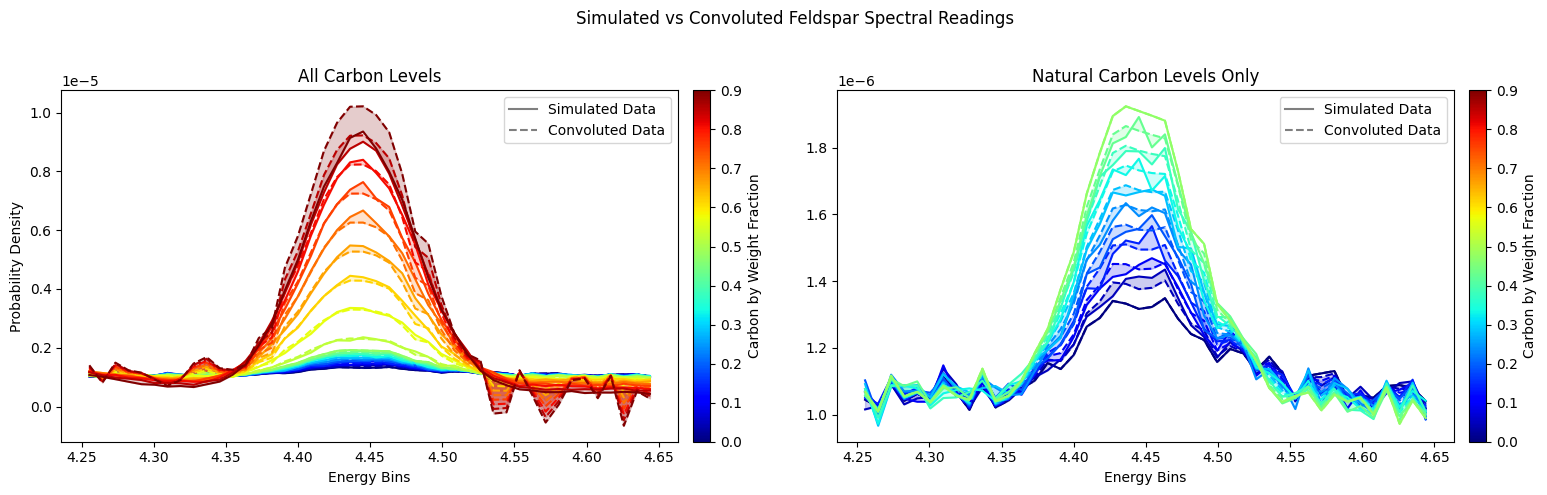
\includegraphics[width=0.8\textwidth]{../Figures/DataGeneration/Sim_vs_Convoluted_FeldsparSpectralReadings_Combined.png}
\caption{Comparison of simulated vs convoluted data for Feldspar spectral readings}
\label{fig:sim_vs_conv}
\end{figure}